\documentclass[12pt, letterpaper, titlepage]{article}

\usepackage{amsmath}
\usepackage{booktabs}
\usepackage{amsthm}
\usepackage{graphicx}
\usepackage[margin=1in]{geometry}
\usepackage{hyperref, url}
\hypersetup{colorlinks = true, linkcolor = blue, citecolor=blue, urlcolor =
  blue}
\usepackage{natbib}
\usepackage{enumitem}
\usepackage{setspace}

\usepackage[pagewise]{lineno}
%\linenumbers*[1]
% %% patches to make lineno work better with amsmath
\newcommand*\patchAmsMathEnvironmentForLineno[1]{%
 \expandafter\let\csname old#1\expandafter\endcsname\csname #1\endcsname
 \expandafter\let\csname oldend#1\expandafter\endcsname\csname end#1\endcsname
 \renewenvironment{#1}%
 {\linenomath\csname old#1\endcsname}%
 {\csname oldend#1\endcsname\endlinenomath}}%
\newcommand*\patchBothAmsMathEnvironmentsForLineno[1]{%
 \patchAmsMathEnvironmentForLineno{#1}%
 \patchAmsMathEnvironmentForLineno{#1*}}%

\AtBeginDocument{%
 \patchBothAmsMathEnvironmentsForLineno{equation}%
 \patchBothAmsMathEnvironmentsForLineno{align}%
 \patchBothAmsMathEnvironmentsForLineno{flalign}%
 \patchBothAmsMathEnvironmentsForLineno{alignat}%
 \patchBothAmsMathEnvironmentsForLineno{gather}%
 \patchBothAmsMathEnvironmentsForLineno{multline}%
}

% control floats
\renewcommand\floatpagefraction{.9}
\renewcommand\topfraction{.9}
\renewcommand\bottomfraction{.9}
\renewcommand\textfraction{.1}
\setcounter{totalnumber}{50}
\setcounter{topnumber}{50}
\setcounter{bottomnumber}{50}

\newcommand{\jy}[1]{\textcolor{blue}{JY: #1}}
\newcommand{\eds}[1]{\textcolor{red}{EDS: (#1)}}


\title{On Sample Size for Block Bootstrap Confidence Intervals 
  to Have Desired Coverage Rates}

\author{Mathew Chandy
%   \href{mailto:mathew.chandy@uconn.edu}
% {\nolinkurl{mathew.chandy@uconn.edu}}\\
  and Jun Yan\\[1ex]
  Department of Statistics, University of Connecticut\\
}
\date{}

\begin{document} 
\maketitle

\begin{abstract}
Block bootstrap is a method that is useful for estimating a parameter of a time
series. Theoretically, the method will work perfectly given an infinitely
large sample of the time series. It is necessary to know how large of a finite
sample is required for block bootstrap estimation to work. Before this study,
there have been no investigations into this problem within the literature. The
aim of this study is to answer this question by simulating replications of
block bootstrap interval estimations of a parameter of a time series, and
recording the rate at which the parameter is recovered by each replicate
interval. The sample length required for acceptable performance is
unsurprisingly found to be dependent on the type of interval construction and
the series' level of temporal dependence.


\bigskip
\noindent{\sc Keywords}:
dependent data; gsimulation
\end{abstract}

\doublespace

\jy{Practice my writing tips on latex (e.g., keep line width under 80; use
  double blank lines to separate paragraphs; etc.):
  \url{
https://statds.github.io/stat-writing/using-the-right-tools-for-writing.html},
  chapter 2}

\jy{turn on the column number mode of your editor. Keep the width to under 80.}


\section{Introduction}
\label{sec:intro}

Block bootstrap is a powerful tool for constructing confidence intervals when
making inferences about dependent data. Early ideas were developed
independently by \citet{hall1985resampling}, \citet{carlstein1986use}, and 
\citet{kunsch1989jackknife}.
It has since been applied in various fields such as econometrics
\citep{mackinnon2006bootstrap} and meteorology \citep{varga2017generalised}.
Block bootstrap is particularly useful for serially dependent
data when the serial dependence is not specified or not of primary interest.
The method is expected to produce confidence intervals with coverage rates
matching their nominal levels as the sample size grows to infinity. However,
when dealing with finite sample sizes, an important question is how large the
sample size needs to be for block bootstrap confidence intervals to have the
desired coverage rates.


The necessary sample size for bootstrap standard errors to provide valid
uncertainty measures in practice has not been extensively studied. For
independent data and non-block bootstrap, \citet{hesterberg2015teachers} notes
that while percentile-based confidence intervals from nonparametric bootstrap
are more accurate than $t$-intervals for larger sample sizes, they are
less accurate for smaller sample sizes. In the contect of structural equation
modeling, \citet{nevitt2001performance} find
that a sample size of 200--1000 is usually sufficient for interval estimation
using standard nonparametric bootstrap. For dependent data, the necessary sample
size for block bootstrap is even less clear. In a linear regression setting with
dependent data, \citet{goncalves2005bootstrap} find that, standard error
estimates from block bootstrap in small samples may be more accurate than
inference from closed-form asymptotic estimates, but block bootstrap percentile
confidence intervals still do not have sufficient coverage even for sample size
$n = 1024$.


The goal of this paper is to provide some practical recommendations on
necessary sample size for block bootstrap with dependent data. We consider a
simple situation of a stationary time series, where the parameters of
interests are the mean, standard deviation, and the first-order
autocorrelation coefficient. We compare three variants of block bootstrap
confidence intervals from the literature \citep{diciccio1996bootstrap,
  rice2006mathematical}: a basic percentile interval, a percentile
interval centered around the estimate, and a bias-corrected and
accelerated ($BC_a$) interval also centered around the original estimate. Their
empirical coverage rates at different sample sizes and dependence levels are
compared in a simulation study. The results of this study suggest that
appropriate recovery of temporal dependence parameters is heavily dependent on
the type of interval used.


The remainder of the papers is organized as follows:
The Block Bootstrap Confidence Intervals section reviews how these intervals
are constructed as well as the general procedure for block bootstrap parameter
estimation. The Simulation Study section offers an explanation of the
simulation design and results. Finally, the Concluding Remarks section
discusses the main takeaways from the results, how these findings could be
useful, and possible future explorations.


\section{Block Bootstrap Confidence Intervals}
\label{sec:blkbootreview}

Consider a stationary time series $\{X_t: t = 1, \ldots, n\}$ with length~$n$.
Our goal is to construct a confidence intervals for a parameter $\theta$ in the
data generating model of the series. Suppose that $\hat\theta_n$ is a point
estimator of~$\theta$ based on the observed series. Bootstrap is a powerful
approach to construct confidence intervals. If the observations in the series
were independent, a standard nonparametric bootstrap procedure would draw a
large number~$B$ bootstrap copies of the observed data, and calculate an
estimate $\hat\theta_n^{(b)}$ for each copy $b = 1, \ldots, B$. The uncertainty
of $\hat\theta_n$ is then estimated by the empirical uncertainty of the
$\hat\theta_n^{(b)}$'s. When serial dependence is present, the bootstrap
procedure needs to preserve the serial dependence. Block bootstrap was motivated
for this situation.

\subsection{Draw a Block Bootstrap Sample}

\jy{Paragraph: describe how to construct one non-overlapping block bootstrap
  sample.}

\jy{Paragraph: describe how to construct one overlapping block bootstrap.}

\jy{Paragraph: comment on selection block size;
  mention that the two procedures are both valid with similar performance (cite
  references to support the claim).}

\subsection{Construct Confidence Intervals}

Suppose that we have repeated the steps in the last subsection $B$ times, and
that for $b \in \{1, \ldots, B\}$, we have obtained an estimator
$\hat\theta_n^{(b)}$ based on the $b$th bootstrap sample using the same method
that was applied to $\{X_t: t = 1, \ldots, n\}$ to obtain $\hat\theta_n$.
Now the question is, how to construct confidence intervals for $\theta$
using the $B$ bootstrap point estimates
$\{\hat\theta_n^{(1)}, \ldots, \hat\theta_n^{(B)}\}$.


\jy{Paragraph: bascic percentiles; use the terminologies in the literature.}

\jy{Paragraph: centered.}

\jy{Paragraph: BCa}




Block bootstrap is a method that can be used to estimate a parameter of
serially dependent data. Suppose that one wants to estimate a parameter or
parameters $\theta$ of a population. The first step is to generate a sample of
length $n$ from the population. An estimate of the parameter
$\hat{\theta}_{n}$ can be computed from this sample. A pseudo-estimate
$\hat\theta_n^*$ can be computed from a bootstrapped pseudo-sample. The mean
$\bar\theta_n^*$ of many replicate $\hat\theta_n^*$ can also be computed.
Lastly, for each $\hat\theta_n^*$, $\delta^* = \hat\theta_n^* -
\bar\theta_n^*$ can be computed.


In basic bootstrap procedure, the new pseudo-sample of size $n$ would be
created by simply resampling observations from the original sample with
replacement. However, in the case of a time series, in order to account for
the temporal dependence, the time series can be split into blocks, typically
of the same size. The block should be of size $l$ large enough for each
pseudo-sample to exhibit some temporal dependence, yet small enough for there
to be some variability between each pseudo-sample. Ideally, as $n$ increases,
$l$ should also increase, but $l / n$ should decrease. To achieve this, $l$ is
often assigned a value as a function of $n$. A common function that is
considered the best by much previous literature is $l = \lceil n^{1/3} \rceil$
\citep{buhlmann1999block}.


The designer of the study can choose whether the blocks overlap or not. If the
blocks do not overlap, it is called non-overlapping or non-moving block
bootstrap. In this case, blocks are resample randomly from the set of all
non-overlapping blocks of size $l$. For non-moving block bootstrap, $l \vert n$
must always be true. In this case, a set of $n / l$ non-overlapping blocks of
size $l$ is constructed from the original sample. Each bootstrapped
pseudo-sample is created by sampling $n / l$ blocks with replacement from the
same set.

If the blocks do overlap, it is called overlapping or moving block bootstrap.
In this case, blocks are resampled randomly from the set of all possible
blocks of size $l$. For moving block bootstrap, $l \vert n$ is not a necessary
condition. The set of available blocks is created by iterating through each
observation $i$ in the original sample and adding to the set the block of size
$l$ that begins with $i$. This set can limited to blocks that end with an
$i <= n$, meaning that $n - l + 1$ blocks are availabe to resample from, or it
can be expanded to include blocks that ``wrap around'': in
other words, blocks that end with a lesser index than the index they began
with, meaning that $n$ blocks are available to resample from. If $l \vert n$,
a bootstrapped pseudo-sample is created by taking a sample of $n / l$ blocks
from the set with replacement to create a new pseudo-sample of size $n$. If
$l does not divide n$, the last block selected will be reduced in size so that
the final size of the pseudo-sample is $n$. Moving block bootstrap was used in
this study as it has been found to yield the lowest error in general
\citep{radovanov2014comparison}. The set of available was not limited as
described above.

An estimate $\hat\theta_n^*$ is computed from the pseudo-sample. This
procedure can be repeated many times to create a distribution of
$\hat\theta_n^*$. 


In this study, 1000 $\hat\theta_n^*$ were created for one simulation of block
bootstrap estimation. Using this distribution of $\hat\theta_n^*$, several
variants of a $1 - \alpha$/2 \% confidence interval for the parameter can be
constructed. The most simplistic method for constructing this interval is the
basic percentile confidence interval. For a parameter $\theta$, the percentile
$1 - \alpha$/2 \% confidence interval takes the form: 
\[ [\hat\theta_{n, \alpha/2}^*, \hat\theta_{n, 1 - \alpha/2}^*].\] 
	
This interval works well when attempting to recover the mean and
standard deviation of a temporally dependent process, but its coverage of
the temporal dependence deteriorates as $n$ increases. A potential solution to
this issue is to center the intervals around $\hat{\theta}_{n}$. To do this,
the distribution of $\delta^*$ should be considered. For a parameter $\theta$,
the $\hat{\theta}_{n}$-centered $1 - \alpha$/2 \% confidence interval takes
the form:
\[ [\hat{\theta}_{n} + \delta^*_{\alpha/2},
  \hat{\theta}_{n} + \delta^*_{1 - \alpha/2}].\] 
  
An alternative method is a $BC_a$ interval centered around $\hat{\theta}_{n}$.
For a parameter $\theta$, the $BC_a$ $1 - \alpha$/2 \% confidence interval
takes the form:
\[ [\hat{\theta}_{n} + \delta^*_{\alpha_1},
  \hat{\theta}_{n} + \delta^*_{\alpha_2}].\] 
$\alpha_{1}$ and $\alpha_{2}$ are the cumulative probability of $z_{1}$ and
$z_{2}$, respectively, where:
\[z_{1} = \frac{z_{0} - z_{1 - \alpha/2}}{1 - a(z_{0} - z_{1 - \alpha/2})} +
z_{0}\] and
\[z_{2} = \frac{z_{0} + z_{1 - \alpha/2}}{1 - a(z_{0} + z_{1 - \alpha/2})} +
z_{0}.\] 
Where $z_0$ is the quantile function of the proportion of
$\hat\theta_n^* < \bar\theta_n^*$, and $a$ is the skewness (computed using
the skewness function from the R e1071 package \citep{e1071}) of
$\hat{\theta}_{n, -i}$, where $\hat{\theta}_{n, -i}$ is the statistic of the
original sample computed without the $i^{th}$ block.


Thus, there are three types of intervals that can be constructed for block
bootstrap estimation in this study: Percentile, $\hat{\theta}_{n}$-Centered,
and $BC_a$. 


\section{Simulation Study}
\label{sec:simstudy}

We designed a simulation study to compare the performance of the different block
bootstrap confidence intervals. In particular, we generated time series $X_t$
from a 1st order auto-regressive (AR1) process:
\[
X_t = \phi X_{t-1} + \epsilon_t,
\]
where $\phi$ is an auto-regressive coefficient, and $\epsilon_t$ is a series of
independent errors from a normal distribution with mean zero and variance
$\sigma_{\epsilon}^2$. The strength of the serial dependence is controlled by
$\phi$, which was set to five levels: $\{-0.4, -0.2, 0.0, 0.2, 0.4\}$.
The series $X_t$ has mean zero and variance
$\sigma_x^2 = (1 - \phi^2) \sigma_{\epsilon}^2$, so for each value of $\phi$, we
set $\sigma_{\epsilon}^2 = 1 / (1 - \phi^2)$ such that $\sigma_x^2 = 1$.


Three target parameters of $X_t$ were considered:
1) $\mu = 0$, the mean of $X_t$;
2) $\sigma_x^2 = 1$, the variance of $X_t$; and
2) $\phi$, the lag-1 auto-correlation coefficient.
To investigate the effect of sample size~$n$, we considered an array of values
$n \in \{100, 200, \ldots, 1000\}$. In each configuration, we genrated 1000
replicates. For each replicate, we constructed three 95\% block bootstrap
confidence intervals for each parameter as described in the last section, and
estimated their actual coverage rates along with their 95\% confidence
intervals from the 1000 replicates. The block bootstrap sampling step was done
with function \texttt{tsboot} from R package \textsl{boot} \citep{boot}, with
block size \jy{size? also it was overlapping blocks. Describe the details here.}
The results are graphically displayed in Figures~\ref{fig:mu}--\ref{fig:phi}.



\jy{One paragraph for each parameter; write down your observations in bullet
  points and then organize them into a logically flowing paragraph.}

\jy{One summary paragraph at the end.}


Each of these 9 intervals either recovers $\theta$ or does not. Remember that
95\% of many of a certain type of 95\% confidence intervals constructed from
samples of the same $n$ should recover $\theta$. To see if this is
approximately the case, one can run 1000 replications of the block bootstrap
procedure, and for each interval-$\theta$ pair, the rate at which that type of
interval recovers $\theta$ can be recorded. The coverage rate is, of course, a
point estimate of a proportion, so a 95\% confidence interval of this coverage
proportion (with $n_{CI} = 1000$) can be constructed, and if the proportion
.95 is included in the interval, the block bootstrap method is likely working
well. If all values in the interval are below .95, the results suggest that the
method either is providing an inaccurate estimation, is underestimating the
process' variability, or a combination of both. If all values in the interval
are above .95, the results suggest that the method is overestimating the
process' variability.


If $\theta$ is not covered at that $n$, a larger $n$ may be
necessary, assuming that performance will improve as $n$ is increased. $n =$
100, 200, 300, 400, and 500, 600, 700 were used in this study. Remember that
the goal of this study is to find the smallest $n$ which is sufficient for
proper coverage. 


The figures below which are grouped by the target $\theta$  were created using
the R ggplot2 package \citep{ggplot2}.


\begin{figure}[tbp]
  \centering
  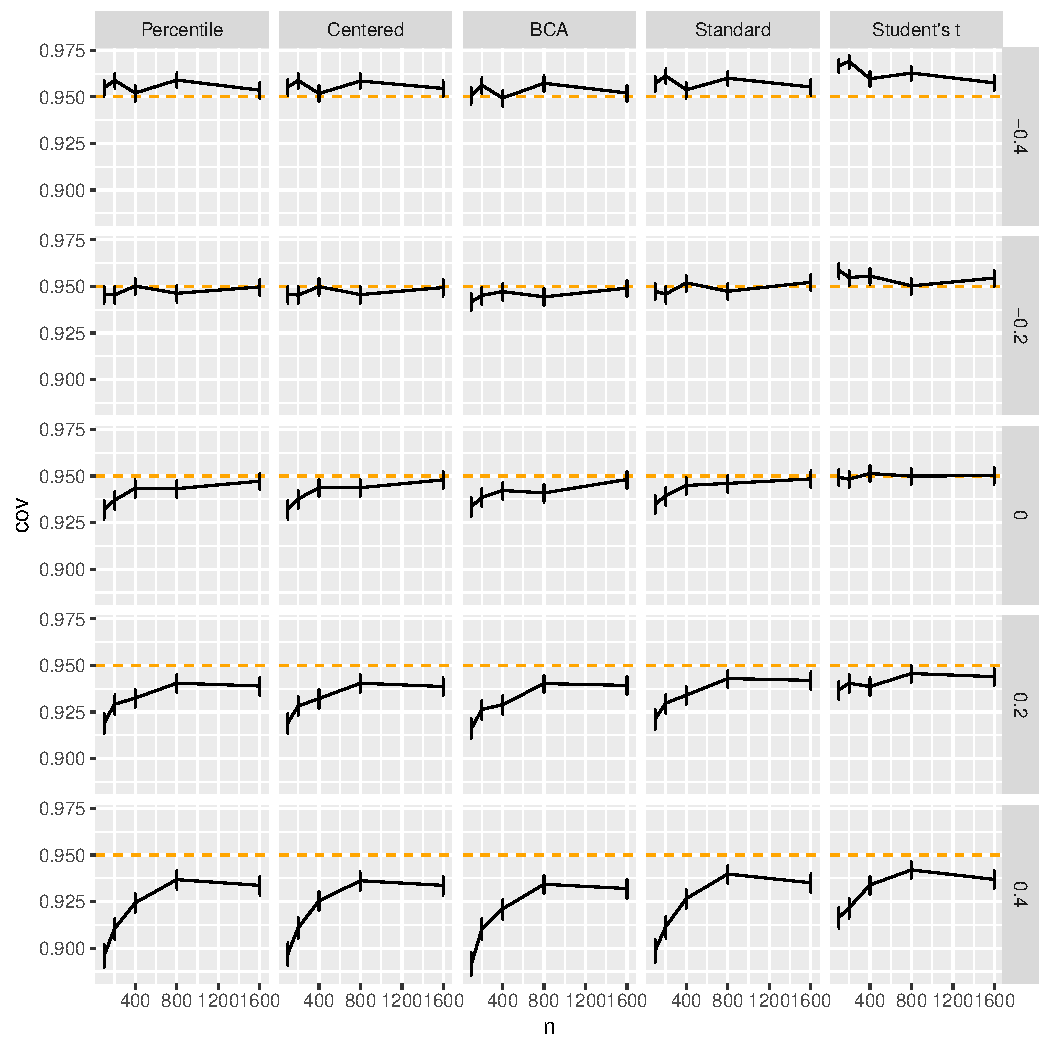
\includegraphics[width=\textwidth]{figures/plot_mu}
  \caption{At $\phi = -.4, -.2$, all intervals seem to cover $\mu$ correctly
    as low as $n = 100$. At $\phi = 0$, an $n$ of 500 seems large enough to
    cover $\mu$ acceptably regardless of interval type. At $\phi = .2$,
    $n = 300$ seems to be sufficient to appropriately recover $\mu$ for all
    intervals. A much larger $n$ seems to be necessary to recover $\mu$ at a
    $\phi$ as high as $.4$.}
  \label{fig:plot_mu}
\end{figure}


\begin{figure}[tbp]
  \centering
  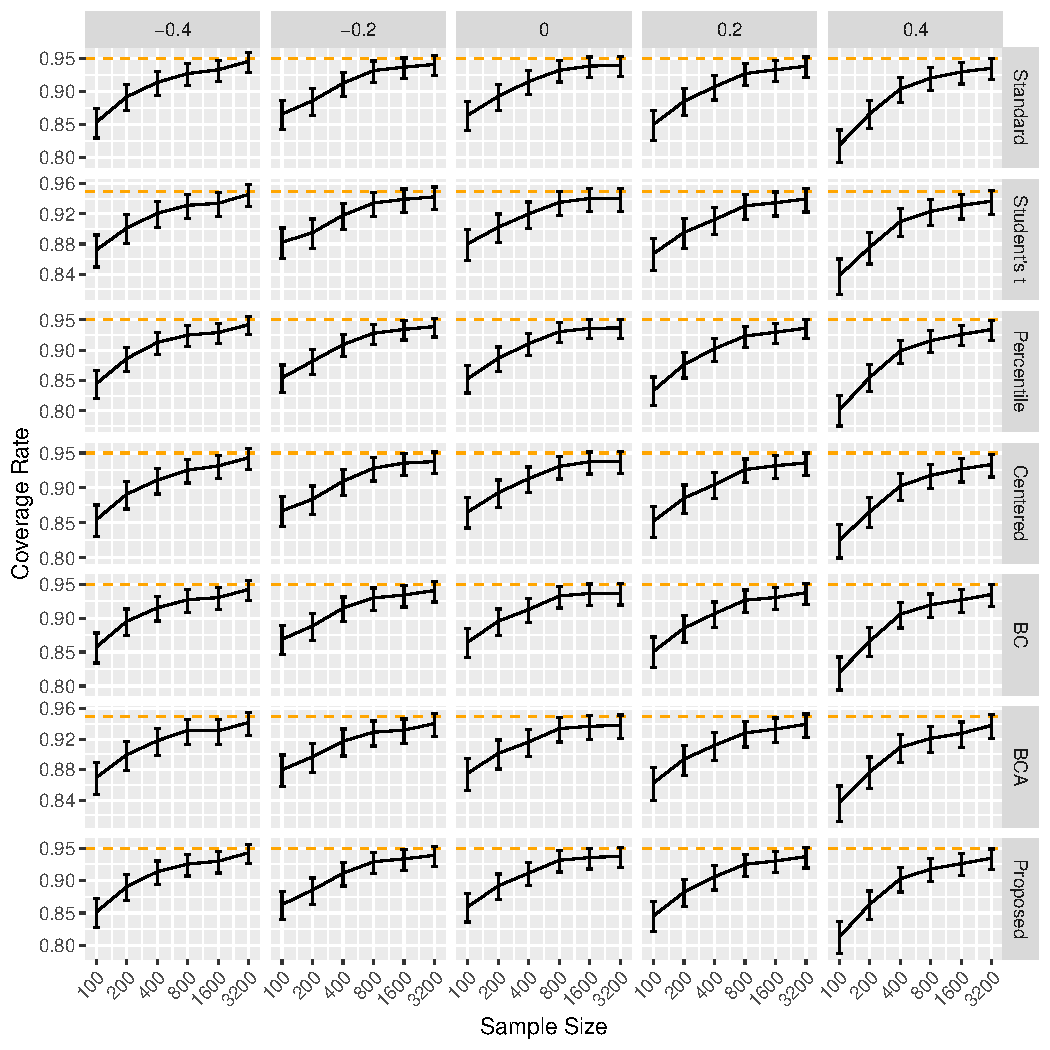
\includegraphics[width=\textwidth]{figures/plot_sigma}
  \caption{At $\phi = -.4$, the percentile and the
    $\hat{\theta}_{n}$-centered intervals recovered $\mu$ well as low as
    $n = 400$, whereas the $BC_a$ interval undercovered $\mu$ for all $n$
    observed. At $\phi = -.2$, the percentile and the
    $\hat{\theta}_{n}$-centered intervals recovered $\mu$ well as low as
    $n = 500$, but the $BC_a$ coverage rates were lower.}
  \label{fig:plot_sigma}
\end{figure}


\begin{figure}[tbp]
  \centering
  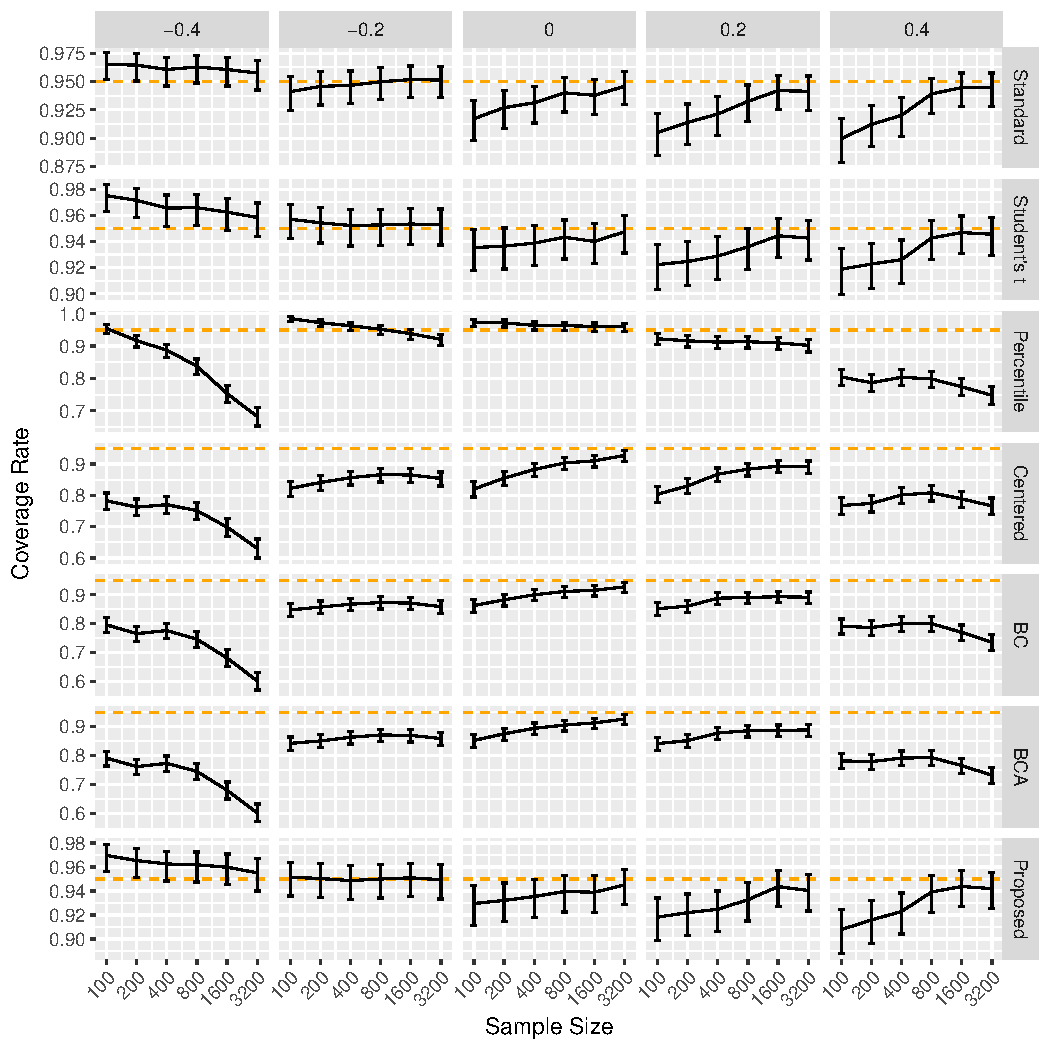
\includegraphics[width=\textwidth]{figures/plot_phi}
  \caption{}
  \label{fig:plot_phi}
\end{figure}


As shown in the above figures, only $\hat{\theta}_{n}$-centered intervals
managed to solve the deterioration problem with respect to recovering $\phi$,
indicating that this interval should be used as opposed to the uncentered
percentile interval or the more complex $BC_a$ interval when estimating
$\phi$. Increasing $n$ will not fix the performance of either of these
intervals because the assumption that the coverage rate will approach an upper
limit of .95 as $n$ increases is invalid. As expected for
$\hat{\theta}_{n}$-centered intervals, a higher positive $\phi$ demands a
larger $n$ to estimate all parameters, but a negative $\phi$ may require a
lesser $n$. For example, for both $\phi = 0.2$ and $0.4$, $n = 100$ was
sufficient to recover $\mu$ at a rate of approximately 95\%.


\section{Concluding Remarks}
\label{sec:conremarks}

\jy{Discussion points:
  1) common practice on block bootstrap even for simple parameter such as the
  mean;
  2) further investigation needed for phi;
  3) impact on applied statsitics courses; student reactions (Dr. Schifano).
}


The motivation for the study is the idea that block bootstrap procedure will
perfectly estimate a parameter of a time series given an infinitely large
sample. The goal for this study was to find what is a good enough finite
sample length for block bootstrap estimation to recover the parameter of a
time series at an acceptable rate. Again, this relies on the assumption that
there is a size $n$ large enough for the method to work: that is, the method's
performance improves as $n$ increases. Out of the two types of intervals used
in this study, this assumption was found to hold true with respect to
estimating $\phi$ only for $\hat{\theta}_{n}$-centered intervals, whereas both
percentile $BC_a$ intervals exhibited coverage deterioration as $n$
increased. When using $\hat{\theta}_{n}$-centered intervals and $\phi$ is
unknown, the results of this study suggest that an $n$ of around 500 may be
necessary to estimate $\mu$, and an $n$ of around 400 may be necessary to
estimate $\sigma$. If $\phi$ is already known, a lesser $n$ may be adequate to
estimate these parameters. When $\phi$ was negative, a $n$ of around 100 was
sufficient to estimate $\mu$. However, in real world applications, $\phi$ is
more commonly found to be positive, so a larger $n$ is more likely to be
necessary. Lastly, to estimate $\phi$, an $n$ of around 400 may be necessary.
This information could prove to be useful for researching using block bootstrap
estimation of time series in domains such as econometrics. Future studies
could investigate if there are types of block bootstrap intervals
constructions that would more appropriately recover the parameters of a time
series. One could also investigate the $n$ needed to make inferences about
other forms of serially dependent data such as an MA process.


\bibliographystyle{chicago}
\bibliography{citations}

\end{document}

